\section{Introduction}
\subsection{Background and engineering problem}
GPU sharing for inference is an operating-system resource-management problem: several services compete for finite execution capacity, device memory and access to a runtime that may not expose the control required by a service-level objective. Increasing concurrent execution can improve aggregate work completed while worsening the response of an individual service. Conversely, reserving the entire accelerator for one model can simplify interference management but leaves less opportunity to use spare capacity. The engineering question is therefore conditional: which mechanism should be selected for a particular workload, latency objective, memory requirement and isolation boundary?

The evidence makes this tension concrete. The ParvaGPU manuscript reports a local configuration in which throughput increases from 354 to 446 requests/s as the number of MPS processes rises from one to three, while reported latency increases from 11 to 27 ms. These outcomes move in opposite desirable directions. The latency quantile is unspecified, so the example cannot establish a P99 service guarantee. XSched instead reports a foreground P99 ratio of 1.07 relative to standalone execution, compared with 1.53 for native Triton in the recorded configuration. These are different engineering objectives, not numbers on one ranking scale \cite{P011,P015}.

\subsection{Scope and contribution}
The unit of technical interpretation is concurrent inference on one physical GPU. A multi-GPU or cluster paper contributes only where a local sharing result can be separated from fleet scheduling. Mixed inference/training papers contribute inference outcomes and the associated background-work cost. Training throughput is not relabeled as inference throughput. Non-GPU accelerator results in otherwise relevant papers are outside the primary comparison.

This working draft integrates the frozen 20-study/21-report corpus with seven source-eligible additions, giving 27 studies represented by 28 reports. Its contribution is a decision-oriented comparison that joins mechanisms, evaluation conditions, reported outcomes, implementation costs and limitations. Existing surveys already examine multi-tenant GPU inference, accelerator-sharing efficiency/fairness/security, and GPU-datacenter scheduling \cite{surveyYu,surveyHuang,surveyYe}. The present taxonomy is therefore an organizational tool, not a first-survey claim. Its narrower emphasis is local GPU outcome traceability, comparability, source-version boundaries and conditional engineering decisions, including relevant 2025 systems. The survey audit records accessed versions and unavailable contextual leads; it does not establish exhaustive novelty. It distinguishes performance interference, resource partitioning, memory protection and fault containment. It also retains adverse outcomes rather than selecting only favorable headline speedups.

The review is not an exhaustive census of the search results. All 559 records in the continuation branch now have a title/abstract-stage decision: 225 exclusions and 334 advancements. Seven additions and two full-text exclusions are resolved; 325 advanced records still await eligibility or report-identity closure. This draft supports candidate selection under observed conditions while the wider coverage question remains open.

\subsection{Objectives}
The objectives are to classify the available mechanisms by their actual control boundaries; determine which outcomes are comparable; explain the conditions behind benefits and regressions; and derive recommendations that identify both expected benefit and sacrifice. The review does not seek a universal winning system. It seeks an auditable reason for choosing a candidate under stated constraints.

\section{Research questions}
The following research questions reproduce the submitted Task 1 protocol (Table 3).
\begin{description}
\item[RQ1] What time-slicing, MPS, MIG and API remoting mechanisms are evaluated for concurrent inference on one GPU, and how do sharing granularity, layer and isolation boundary classify them?
\item[RQ2] How do studies measure utilization, throughput, density, average/tail latency, predictability and interference, and how comparable are their experimental methods?
\item[RQ3] Under what GPU, workload, batch, tenant mix and configuration conditions are changes in utilization, throughput, density and latency reported?
\item[RQ4] What resource and fault isolation properties, trade-offs, implementation costs and conflicting results are reported, and what limits the evidence?
\item[RQ5] Which approach or combination is supported for specified inference-serving conditions and priorities, with what confidence and alternatives?
\end{description}

\section{Research methodology}
\subsection{Protocol and implemented method}
The submitted Task 1 protocol is preserved unchanged in the repository. It specifies independent screening and appraisal, stable record/report/study identifiers, page-level extraction and a condition-aware narrative synthesis. This draft follows its conceptual comparison rules while explicitly reporting deviations in execution. PRISMA supplies the reporting framework, while the search audit preserves the executed queries rather than replacing them with planned expressions \cite{prisma,prismas,kitchenham}.

The supplied Task 2 workbook is the source of the current corpus and historical decisions. GitHub's preceding status described an earlier 15-form assessment. Importing the newer workbook does not mean those older registers were silently rewritten. Task 3 stores the uploaded baseline separately and keeps the inherited research history available.

The implemented review uses a single automated source-based assessment under team direction. For the continuation, the user reported instructor permission to rely fully on this process; amendment M2026-10-23 records that oral permission as user-reported, rather than independently inspected written approval. No independent human item-level votes or calibration are inferred. Activity records preserve actual preparation and decision times, which do not establish when a person reviewed a record.

\subsection{Integrated source review of all included studies}
The frozen source-review packages cover the original 20 studies and the REEF companion report: 70 appraisal items and 30 outcomes for Eshaal's allocation, 70 appraisal items and 13 outcomes for Raazia's, and 60 appraisal items and nine outcomes for Rameen's. All 200 appraisal items, 126 included-report inclusion-criterion checks and 52 retained outcomes have source-anchored review entries. The original baseline forms are preserved separately. The 12 inherited criterion checks for the two excluded reports are not recertified by this included-study review.

Corrections include GPU-specific VastPipe context; final iGniter anchors; gpulets' model-pair statistic; REEF conference/journal boundaries; Clockwork's TVM v0.7 environment; Torpor's evaluation/deployment distinction; KRYPTON's two-stage arrival-rate setup; XSched's Section 8 anchor; InferFair's goodput and slowdown-fairness definitions; ArkGPU's adverse result; Dyna-P's local sensitivity experiment; KRISP's AMD emulation; and Tally's total normalized system throughput. The supplied InferFair copy closes the last missing included-study source.

A common claim-specific Q9 appraisal distinguishes directly tested performance protection from untested security/fault guarantees. The gpulets artifact appendix also supports a higher reporting/reproducibility score without claiming local reproduction. The original 20-study scores sum to 338/396 applicable points; this aggregate describes reporting appraisal and must not be interpreted as an effect size or certainty rating. Original, source-reviewed and independent human fields remain separate. ParvaGPU numerical evidence is still specific to arXiv v1; final-text equivalence is not established. This integration does not supply independent human votes.

The continuation adds 42 source-anchored inclusion-criterion judgments, 70 Q1--Q10 items and 18 outcome rows for LithOS, Abacus, Miriam, SGDRC, Pantheon, Oneiros and GACER. The first six appraisal totals are17,17,16,16,16and17out of20; GACER scores13/18with a reasonedN/A isolation item. Combined with the original forms, the working corpus has 270 appraisal items, 168 included-report inclusion checks and 70 outcome rows. The study-level appraisal sum is 450/534 applicable points. This accounting describes reporting quality, not independent replication or a certainty-weighted effect. The seven additions and their anchors appear in Appendix~\ref{app:additions} \cite{s021,s022,s023,s024,s025,s026}.

\subsection{Databases, search fields and period}
The active occurrence register represents ACM Digital Library, IEEE Xplore, Springer Nature Link and ScienceDirect, with supplementary named-paper lookups recorded separately. Their relevance is complementary: systems conferences, parallel/distributed systems research and journal literature provide different routes to sharing mechanisms. However, representation in an imported register is not equivalent to verified complete coverage of every planned database run.

The main publication window is 2020 through the date of each executed search in October 2026. IEEE and Springer entries record 11 October; ACM and ScienceDirect entries record 14 October. Later retrieval of a paper does not change an earlier search cutoff. The older journal survey used as an organizational benchmark is contextual literature, not an additional included primary study.

The executed expressions generally combine GPU terms, inference/model-serving terms and mechanism terms. Some interfaces use broad indexed fields rather than title/abstract/keywords. Broad fields can retrieve papers in which sharing terminology occurs only in references or background. Conversely, restricted inference expressions can miss papers described only as LLM serving. The exact retained expressions, fields and filters are reproduced in Appendix~\ref{app:search}; the workbook holds filenames and provenance.

The historical ACM master record contains displayed, claimed and parsed totals of 1,600, 1,603 and 1,829. The ScienceDirect MPS record retains 517 displayed against 563 registered. These differences are not corrected by inventing a missing export or changing a count to match another artifact. The active consolidated occurrence totals and their original discrepancies are different fields.

\subsection{Eligibility and study identity}
All inclusion criteria must be met: an English peer-reviewed primary report; evaluated concurrent sharing on one physical GPU; inference outcomes, separable where training is also present; interpretable outcomes and configuration; sufficient local technical evidence; and the specified publication period or justified older exception. A paper's title or prestigious venue alone does not establish eligibility.

Decisive exclusion categories are non-primary/non-peer-reviewed material, no evaluable inference-sharing mechanism, hardware-only work without evaluated systems sharing, aggregate-only multi-GPU evidence, non-GPU scope, insufficient assessed technical detail, and period/language mismatch. The supplied source assessment excludes TGS and HiveD because the extracted evaluation concerns training rather than eligible inference-sharing outcomes. These exclusions are kept outside the included-paper catalogue.

Records, reports and studies are distinct entities. A repeated database occurrence is linked during deduplication. A report version remains identifiable even when it belongs to the same underlying study as another report. REEF's conference report P005 and journal extension P023 map to S005; the journal's first page explicitly states the extension relationship \cite{P005,P023}. They cannot supply two independent replications. Other manuscript copies retain their version labels rather than automatically inheriting final-publication page numbers.

\subsection{Appraisal and extraction}
The Q1--Q10 rubric scores 0, 1 or 2 for objective clarity, mechanism description, experimental transparency, hardware/workload description, baseline fairness, utilization/throughput evidence, latency measurement, multi-tenant interference, isolation evaluation and replication/limitations. Justified not-applicable items reduce the applicable denominator. Scores are reporting and internal-validity appraisals, not journal-prestige scores or automatic exclusion criteria.

There are 270 appraisal items for 27 study-level forms: 200 inherited items and 70 new source-based items. After the source-based denominator review, two items are N/A: P001 Q7 and P006 Q9. XSched Q9 is applicable to its directly evaluated performance protection. The frozen baseline retains its original three N/A items. The normalized score is the recorded sum divided by the applicable maximum. The workbook recalculates these sums from the item rows and checks them against the study table. A companion report does not create an additional independent study-level appraisal.

Extraction preserves mechanism, environment, workload, tenants, load/SLO, baseline, result, isolation dimensions, overhead, limitations, source and anchor. The 70 outcome rows and two calculations are not 68 studies. Missing values remain missing or explicitly not established. A throughput ratio is not converted into utilization percentage, a model-pair distribution is not treated as a request-latency percentile, and a reported maximum is not recast as an average.

\subsection{Synthesis and robustness rules}
The synthesis is narrative and comparative. A numerical contrast is interpreted within the source experiment unless GPU, model, batch, load, concurrency, metric and baseline are sufficiently aligned across studies. No pooled speedup or weighted cross-study average is calculated. A result is first evaluated for relevance to the decision, then for comparability and appraisal limitations.

The protocol's below-60\% sensitivity view removes no current study because all recorded normalized scores are at least 70\%. Consequently, an unchanged answer under this cutoff is mechanically expected. It does not demonstrate robustness to publication bias, title-only screening, a different stopping rule or correlated single-reviewer error. Claim-level anchors and version checks remain necessary even for high-scoring studies.

\section{PRISMA study selection and corpus}
The frozen selection logs reconcile 4,189 occurrences minus 114 duplicate links to 4,075 canonical records. Their historical partition is 3,493 screening exclusions, 559 retained records not advanced, 21 included reports and two source-assessed exclusions. That snapshot is preserved separately and is not overwritten by the continuation.

The 559-record branch now has final title/abstract-stage decisions: 225 excluded and 334 advanced. A conservative scope audit reopened 56 earlier proposed exclusions. Of the screening exclusions, 108 explicitly use title/metadata evidence alone. No record is excluded because an abstract is missing. The queue contains 235 original abstract texts plus 161 supplemental recovered texts; 163 records still lack abstract text, and five recovered texts have quality flags.

Of the 334 advanced records, seven new reports met all inclusion criteria and two were excluded at full text under EC2. In-Mig evaluates cross-venue agent reasoning and routing without an extractable GPU-sharing intervention; ALL-RP evaluates social-media repost prediction, with GPU use for model training rather than concurrent inference sharing. The remaining 326 records require eligibility or identity closure. They are neither full-text exclusions nor reports declared unavailable. Duplicate and companion-report proposals remain separate identity checks.

The working included set is therefore 28 reports representing 27 studies, preserving the REEF P005/P023-to-S005 linkage. These counts do not by themselves finalize whole-review PRISMA: historical record/report mapping, source-assessment events and pending identities must be reconciled before a complete final flow is claimed. Later retrieval dates do not change the original search cutoffs. The minimum-study target is met; it is not a cap or a reason to omit further eligible studies.
\begin{longtable}{>{\raggedright\arraybackslash}p{0.7\textwidth}>{\raggedright\arraybackslash}p{0.15\textwidth}}
\toprule
\textbf{Accounting scope / stage} & \textbf{Count}\\\midrule\endhead
Historical identified occurrences & 4,189\\\addlinespace
Historical duplicate links & 114\\\addlinespace
Historical canonical records & 4,075\\\addlinespace
Historical original included reports / studies & 21 / 20\\\addlinespace
Continuation records screened & 559\\\addlinespace
Continuation screening exclusions & 225\\\addlinespace
Continuation advanced to retrieval / eligibility & 334\\\addlinespace
Continuation full-text inclusions / exclusions & 7 / 2\\\addlinespace
Advanced records with unresolved eligibility or identity & 326\\\addlinespace
Working included reports / unique studies & 28 / 27\\\addlinespace
\bottomrule\end{longtable}
\textbf{Stage distinctions:} $559=225+334$ and $334=7+2+325$. Advancement does not mean that all 334 reports have been retrieved or assessed. This is branch accounting, not a completed whole-review PRISMA flow.

\begin{figure}[p]\centering
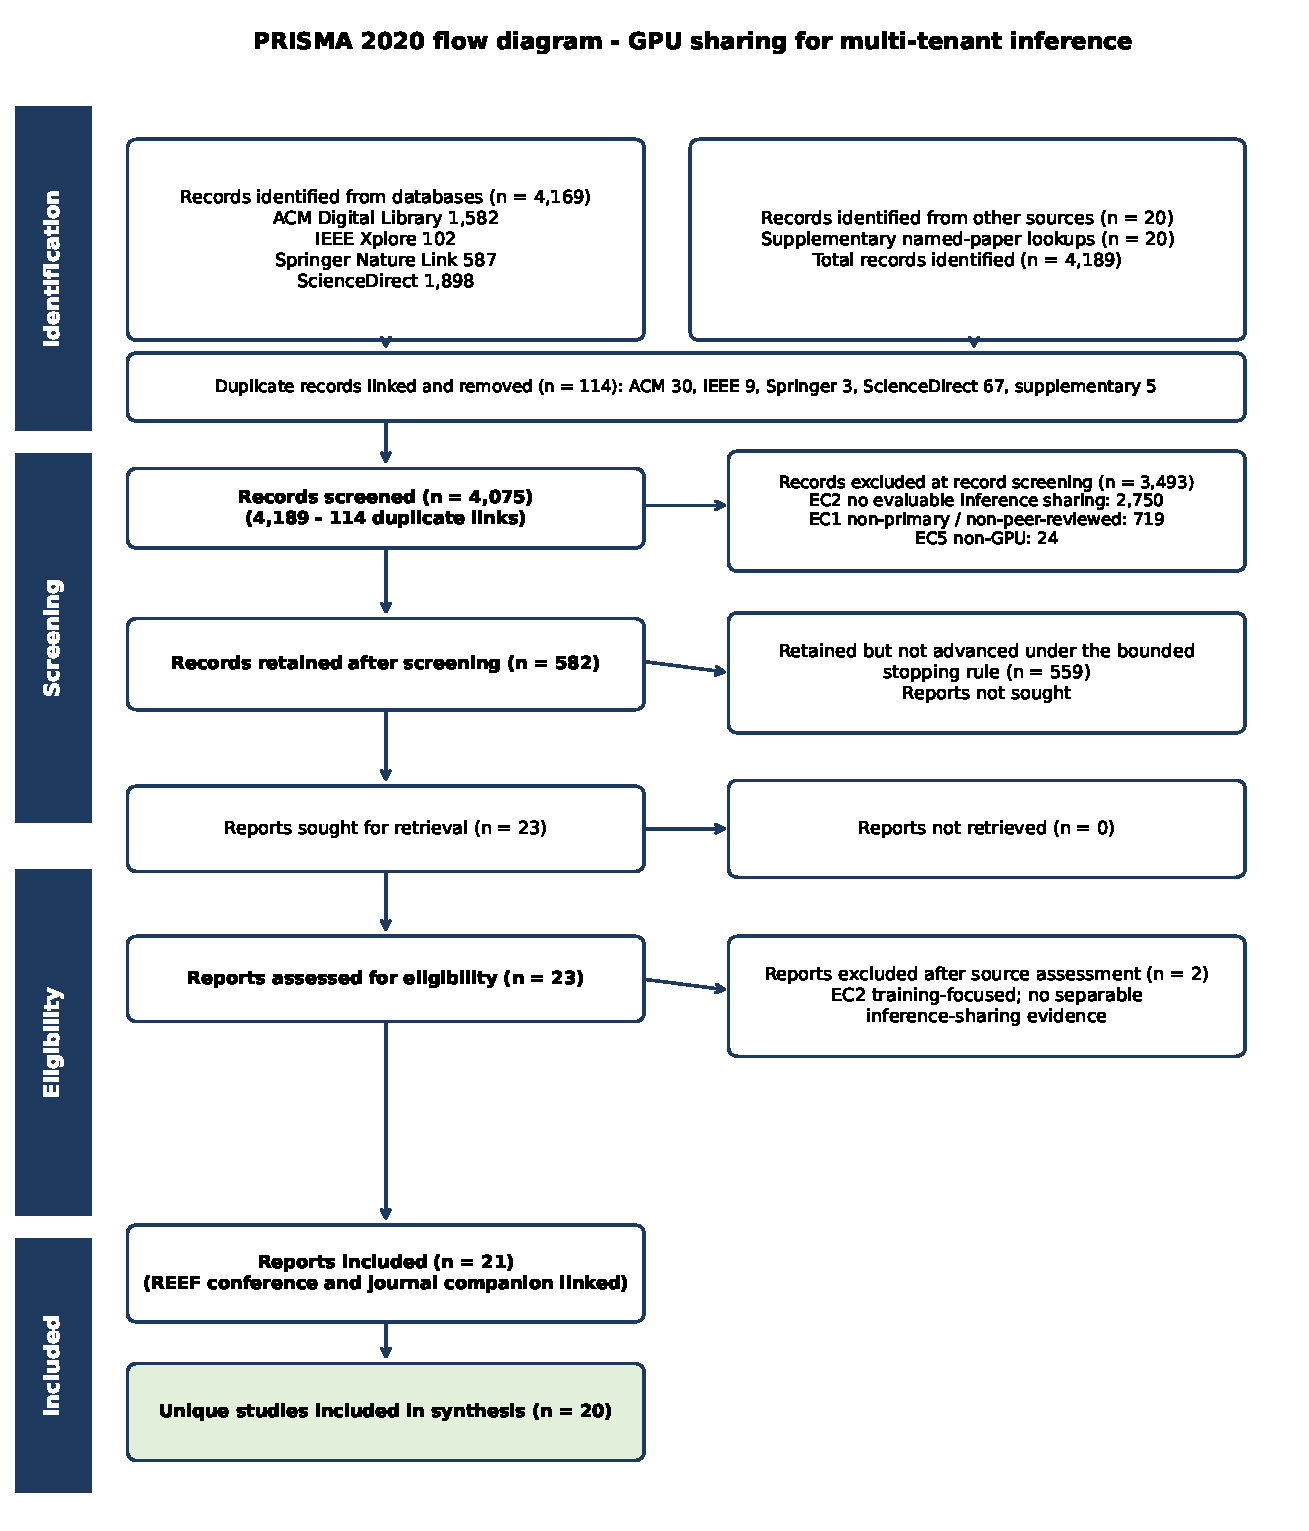
\includegraphics[width=\textwidth,height=.82\textheight,keepaspectratio]{figures/Frozen_PRISMA.pdf}
\caption{Frozen Task 2 selection flow, shown as historical provenance only. The adjacent branch table records later decisions; a reconciled final whole-review PRISMA flow remains pending.}
\end{figure}
\begin{longtable}{>{\raggedright\arraybackslash}p{0.16\textwidth}>{\raggedright\arraybackslash}p{0.62\textwidth}>{\raggedright\arraybackslash}p{0.1\textwidth}}
\toprule
\textbf{Study / report} & \textbf{System / source identity} & \textbf{QA}\\\midrule\endhead
S001 / P001 & VastPipe (2025) & 13/18\\\addlinespace
S002 / P002 & iGniter (2023) & 18/20\\\addlinespace
S003 / P003 & gpulets (2022) & 20/20\\\addlinespace
S004 / P004 & PipeSwitch (2020) & 17/20\\\addlinespace
S005 / P005 & REEF conference (2022) & 18/20\\\addlinespace
S006 / P006 & Paella: Low-latency Model Serving with Software-defined GPU Scheduling (2023) & 16/18\\\addlinespace
S007 / P007 & Orion: Interference-aware, Fine-grained GPU Sharing for ML Applications (2024) & 19/20\\\addlinespace
S008 / P008 & GSLICE: Controlled Spatial Sharing of GPUs for a Scalable Inference Platform (2020) & 17/20\\\addlinespace
S009 / P009 & Serving DNNs like Clockwork: Performance Predictability from the Bottom Up (2020) & 18/20\\\addlinespace
S010 / P010 & Colocating ML Inference and Training with Fast GPU Memory Handover (SIRIUS) (2025) & 17/20\\\addlinespace
S011 / P011 & ParvaGPU: Efficient Spatial GPU Sharing for Large-Scale DNN Inference in Cloud Environments (2024) & 14/20\\\addlinespace
S012 / P012 & Torpor: GPU-Enabled Serverless Computing for Low-Latency, Resource-Efficient Inference (2025) & 15/20\\\addlinespace
S013 / P013 & StreamBox: A Lightweight GPU SandBox for Serverless Inference Workflow (2024) & 17/20\\\addlinespace
S014 / P014 & Efficient Performance-Aware GPU Sharing with Compatibility and Isolation through Kernel Space Interception (KRYPTON) (2025) & 16/20\\\addlinespace
S015 / P015 & XSched: Preemptive Scheduling for Diverse XPUs (2025) & 18/20\\\addlinespace
S016 / P018 & InferFair: Towards QoS-aware scheduling for performance isolation guarantee in heterogeneous model serving systems (2024) & 17/20\\\addlinespace
S017 / P019 & ArkGPU: enabling applications' high-goodput co-location execution on multitasking GPUs (2023) & 16/20\\\addlinespace
S018 / P020 & Dyna-P: placement-aware dynamic partitioning for lightweight applications with modern GPUs (2025) & 15/20\\\addlinespace
S019 / P021 & KRISP: Enabling Kernel-wise RIght-sizing for Spatial Partitioned GPU Inference Servers (2023) & 18/20\\\addlinespace
S020 / P022 & Tally: Non-Intrusive Performance Isolation for Concurrent Deep Learning Workloads (2025) & 19/20\\\addlinespace
S021 / P024 & LithOS (2025) & 17/20\\\addlinespace
S022 / P025 & Abacus (2021) & 17/20\\\addlinespace
S023 / P026 & Miriam (2023) & 16/20\\\addlinespace
S024 / P027 & SGDRC (2025) & 16/20\\\addlinespace
S025 / P028 & Pantheon (2024) & 16/20\\\addlinespace
S026 / P029 & Oneiros (2025) & 17/20\\\addlinespace
S027 / P030 & GACER (2024) & 13/18\\\addlinespace
\bottomrule\end{longtable}

\section{Taxonomy of existing approaches}
A useful taxonomy separates the resource being controlled from the software layer implementing the policy. The same system may appear in more than one category. A MIG-based system can also use MPS; an API interceptor can enforce temporal scheduling; and memory handover can support mixed-workload co-location. Treating these as mutually exclusive labels would hide the source of the observed behavior.

\subsection{Temporal and priority control}
Temporal mechanisms decide which work runs and when another tenant can make progress. PipeSwitch emphasizes switching and model state, Clockwork emphasizes predictable execution and admission, while REEF, Paella, Orion and XSched expose different scheduling/preemption boundaries. Their integration costs and latency meanings differ. PipeSwitch's additional switching-related latency is not interchangeable with XSched's foreground P99 ratio or Paella's reported P99 reduction \cite{P004,P005,P006,P007,P009,P015}.

LithOS extends temporal control with transparent kernel atomization and TPC allocation; Abacus makes operator overlap deterministic so a controller can predict concurrent-service latency. Miriam and Pantheon target edge inference, but at different intervention boundaries: elastic kernels versus chunk preemption combined with early-exit variants. They are not interchangeable implementations of the same scheduler \cite{s021,s022,s023,s025}.

\subsection{Spatial allocation and partitions}
MPS-based allocation and software right-sizing regulate concurrent access to execution resources. VastPipe, iGniter, gpulets and GSLICE provide different allocation, profiling and feedback approaches. KRISP contributes AMD-oriented kernel right-sizing evidence and should not be relabeled as a measurement of NVIDIA MPS. Partition-aware designs, including ParvaGPU and Dyna-P, additionally make placement, profile size or reconfiguration relevant \cite{P001,P002,P003,P008,P011,P020,P021}.

A spatial allocation is only one part of a service guarantee. The model must fit memory, the workload must remain within the profiled regime and the selected resource shares must satisfy its timing requirements. Hardware allocation boundaries do not by themselves establish all possible security or fault guarantees in the reviewed experiments.

\subsection{API, runtime and memory mediation}
Torpor, StreamBox, KRYPTON, ArkGPU and Tally intervene at different points between the application and accelerator. Their common advantage is control over resource use without necessarily changing the model's high-level purpose. Their differences include intercepted interfaces, compatibility, runtime sharing, host work and the degree to which tenants share memory or trust assumptions. SIRIUS contributes a specific memory-handover mechanism for co-located inference and training \cite{P010,P012,P013,P014,P019,P022}.
SGDRC dynamically controls compute and VRAM-bandwidth contention through software mechanisms, while Oneiros remaps model-parameter memory and overlaps CPU/GPU transfers to relieve multi-model memory pressure. Oneiros evaluates temporal and spatial configurations; its memory-management benefit is not a new fault-containment guarantee. SGDRC explicitly reports that its shared CUDA context cannot isolate DNN GPU-runtime failures \cite{s024,s026}.

\begin{longtable}{>{\raggedright\arraybackslash}p{0.25\textwidth}>{\raggedright\arraybackslash}p{0.35\textwidth}>{\raggedright\arraybackslash}p{0.28\textwidth}}
\toprule
\textbf{Family / reports} & \textbf{Control and condition} & \textbf{Cost}\\\midrule\endhead
Temporal / priority; P004 P005 P006 P007 P009 P015 P022 & Request, model, kernel or launch order. A suitable interception/preemption boundary exists & Switch cost, profiling and background slowdown\\\addlinespace
Software spatial sharing; P001 P002 P003 P008 P021 & MPS quota or AMD CU-mask control. Concurrent jobs fit memory and selected compute allocation & Residual interference; quotas are not proof of security\\\addlinespace
Hardware partition and hybrid; P011 P014 P020 & MIG profiles plus temporal/MPS policy. Supported partition profiles fit model memory & Fragmentation, placement and reconfiguration cost\\\addlinespace
API / runtime mediation; P006 P012 P013 P014 P019 P022 & User API, shared runtime or kernel interface. Required APIs and integration hooks are supported & Compatibility, CPU/transfer cost and trust boundary\\\addlinespace
Memory handover; P010 & Inference/training memory ownership. Training can yield memory without breaking inference & Reclamation and integration overhead\\\addlinespace
Fairness policy; P018 & Relative model slowdown and SLO goodput. Comparable per-model service objectives & Not equivalent to request-tail or hostile-tenant isolation\\\addlinespace
Fine-grained temporal / spatial control; P024 P025 P026 & TPC/atomization, deterministic operator overlap and elastic kernels; compatibility and profiled workload assumptions & Kernel support, profiling, latency versus throughput\\\addlinespace
Software compute/bandwidth control; P027 & SM allocation and software VRAM-bandwidth control; shared CUDA context & No DNN runtime-fault isolation\\\addlinespace
Model-adaptive edge preemption; P028 & Chunk preemption plus early-exit variants; permitted accuracy/memory budget & Deadline behavior changes both model work and scheduler cost\\\addlinespace
Parameter-memory virtualization; P029 & Temporal/spatial multi-model service with asynchronous transfer; high CPU/GPU bandwidth & Transfer overhead, memory policy and isolation claims separate\\\addlinespace
\bottomrule\end{longtable}\paragraph{Cross-stack extension.} GACER belongs to compiler/runtime coordination: spatial microbatch splitting and temporal cross-model scheduling complement native streams. This resource-efficiency control does not assert a fault/security boundary \cite{s027}.


\section{Results and evidence synthesis by research question}
\subsection{RQ1: mechanisms and control boundaries}
The corpus supports a layered answer rather than a product list. Temporal control manages ordering and interruption; software spatial control manages concurrent allocation; hardware partitioning constrains resource placement; and API/runtime mediation supplies an enforcement layer. Fairness-aware policy adds a decision objective across these mechanisms. InferFair, for example, is best understood through relative slowdown and useful service, not as a new hardware partition primitive \cite{P018}.

This taxonomy explains why naming MPS, MIG or remoting is insufficient for engineering selection. A deployment also needs a policy, a mechanism for enforcing it and an explicit boundary of protection. The corpus demonstrates several combinations, but its bounded selection does not support a claim that one category is most prevalent in the entire literature.

The seven additions reinforce the layered taxonomy. LithOS coordinates TPC scheduling and atomization, Abacus coordinates operator overlap, Miriam transforms kernels, Pantheon combines chunk preemption with model adaptation, SGDRC controls compute and memory bandwidth, and Oneiros controls parameter-memory residency. The enforcement point and shared state explain which mechanisms can be composed and which integration assumptions must be checked \cite{s021,s022,s023,s024,s025,s026}.

\subsection{RQ2: measurements and comparability}
The outcome register includes requests/s, normalized throughput, goodput, P99/P98 latency, unspecified latency, SLO-violation rate, API overhead, host memory and a composite utilization-efficacy score. These measure different properties. Goodput counts work that meets a service objective, while aggregate throughput may include best-effort work that does not protect the foreground service. A numerical increase in the latter cannot establish improvement in the former.

GSLICE's GUE value of 94.04 is a composite score, not 94.04\% GPU utilization. Its negative signed latency improvement is retained as an unfavorable observation. The gpulets threshold covering 90\% of tested model pairs concerns a distribution across pairs, not the 90th percentile of requests. These distinctions prevent apparently precise but invalid conclusions \cite{P003,P008}.

The reported iGniter prediction-error range of 1.53--5.02\% assesses prediction accuracy, not a latency speedup. Clockwork's approximately 800 requests/s is goodput in a particular evaluation, and the supplied extraction notes a nonidentical comparator setup. Both observations are useful, but neither supports a direct ranking against a throughput ratio measured on another platform \cite{P002,P009}.

Pantheon's deadline-adjusted relative accuracy treats a late job as zero accuracy; it is not ordinary classification accuracy. Abacus excludes deadline-dropped queries from latency calculations while including them in QoS violations, so latency must be read with the violation population. Oneiros separates P99 time-to-first-token (TTFT), including queuing, from time-between-token (TBT), and reports throughput in generated tokens/s. None is directly interchangeable with DNN requests/s or an unspecified latency statistic \cite{s022,s025,s026}.

\subsection{RQ3: conditions affecting results}
Three conditions recur in the evidence. First, concurrency and resource shares affect both completed work and waiting time. The local ParvaGPU contrast shows a throughput benefit accompanied by increased latency. Second, model state and memory transfer can dominate. Torpor's late binding is attractive for low-rate functions, but its density result does not establish that frequent transfers of large models meet the same latency objective. Third, the workload's priority structure determines which sacrifice is acceptable \cite{P011,P012}.

For a foreground-priority service, XSched's 1.07x standalone P99 is relevant because it directly expresses foreground interference in the evaluated setup. Orion's up-to-7.3x aggregate-throughput result describes total work and must be read with its foreground-latency condition. These results can support different decisions without contradicting each other \cite{P007,P015}.

Mixed-workload evidence requires an additional separation. SIRIUS reports an average P99 inference improvement factor of 12.6 against the authors' adapted TaskSwitch baseline. It is not a uniform per-model gain or a direct comparison against unmodified PipeSwitch. ArkGPU's recorded inference/training pairs meet a twice-solo P99 target, while a low-contention setting can lose about 5\% QPS. The unfavorable condition belongs in the synthesis because it changes when the mechanism is worthwhile \cite{P010,P019}.

Miriam's RTX2060 and edge-device results differ by workload and arrival mode; the introductory latency-overhead summary is not a universal bound for the body experiments. Pantheon reports 0.39--1.10\% deadline misses for three stated application mixes, but does so with model-variant, memory and accuracy constraints. Oneiros's C1 spatial-sharing comparison reports author-averaged reductions of 65.5\% in P99 TBT and 20.7\% in P99 TTFT, with 6.6\% higher tokens/s, under the stated trace and model mix. These are within-source conditions, not transferable service guarantees \cite{s023,s025,s026}.

\subsection{RQ4: isolation and implementation cost}
Performance isolation asks whether another workload changes service behavior. Resource isolation asks what capacity is allocated or separated. Memory protection and fault containment concern different failure or adversarial models. A scheduler that limits slowdown is not thereby a complete hostile-tenant security boundary. The extraction cards preserve these dimensions separately, and untested boundaries remain unestablished.

Implementation costs also operate at different levels. API mediation can add host-side work or per-call delay. Model swapping adds transfer and memory pressure. Kernel-space interception introduces compatibility and maintenance requirements. Temporal granularity changes the trade-off between scheduling work and waiting time. The KRYPTON extraction reports an average QoS violation rate of 1.23\% relative to a solo P99 threshold, which is a threshold-relative request fraction rather than a latency in milliseconds. Its original Poisson rate is half the solo maximum; the shared test halves that rate again while assigning 50\% time \cite{P014}.

SGDRC's shared-context execution provides performance control without DNN runtime-fault isolation. Pantheon prioritizes deadlines by trading some model accuracy and memory residency for schedulability, and adds device power relative to its comparator. Abacus incurs profiling and predictor work. LithOS requires compatible interception and kernel behavior; Oneiros relies on high CPU/GPU transfer bandwidth and must cap remapping to avoid extra latency. These costs should be compared to the deployment's constraint, not collapsed into a single isolation or overhead score \cite{s021,s022,s024,s025,s026}.

\subsection{RQ5: conditional selection}
The evidence supports a sequence of decisions. Specify the service objective and trust boundary first. Eliminate mechanisms incompatible with hardware, model memory or required integration. Compare the remaining candidates under the relevant arrival process, batch and co-tenant mix. Measure both protected service and work sacrificed. If the available studies do not cover the required boundary, the appropriate conclusion is insufficient evidence for that guarantee, not an assumed benefit.

The recommendation matrix in Section~10 connects each scenario to report IDs, expected benefits, costs and alternatives. These are evidence-supported candidates for evaluation, not claims that the reviewed implementation can be deployed unchanged in every environment.

The added evidence broadens the candidate set without changing the selection rule. For predictable co-located DNN service, deterministic overlap or fine-grained priority control is a candidate when profiling and compatible kernels are acceptable. For an edge deadline objective, model-changing approaches require an explicit accuracy budget. For memory-constrained multi-LLM service on a high-bandwidth CPU/GPU system, parameter remapping is a candidate while transfer cost remains tolerable. Fault-sensitive or mutually untrusted tenants require a separately established boundary \cite{s021,s022,s023,s024,s025,s026}.

\section{Comparative analysis}
The comparison distinguishes direct within-source contrasts from unmatched cross-study observations. The strongest numerical statements are tied to their original comparator. Even these require attention to whether the result is an average, maximum, lower bound or threshold-relative statistic. An improvement described as ``up to'' is not the expected result for an arbitrary deployment.

\begin{longtable}{>{\raggedright\arraybackslash}p{0.26\textwidth}>{\raggedright\arraybackslash}p{0.28\textwidth}>{\raggedright\arraybackslash}p{0.34\textwidth}}
\toprule
\textbf{Evidence / class} & \textbf{Observation} & \textbf{Interpretation and missing control}\\\midrule\endhead
CMP01 P011 E036 E037 C001 C002. Within-source trade-off & 354 to 446 requests/s; 11 to 27 ms & 25.99\% throughput increase accompanies 2.4545x latency. Missing: Latency quantile; final version equivalence\\\addlinespace
CMP02 P001 E001; P011 E036. Unmatched cross-study & 2.7x versus 25.99\% increase & Different baseline and GPU/model context prevent ranking. Missing: Matched workload, batch and resource budget\\\addlinespace
CMP03 P007 E029 E030; P015 E044. Different objectives & Up to 7.3x aggregate work versus 1.07x foreground P99 & Foreground delay and total completed work must be assessed together. Missing: Common model mix and background progress metric\\\addlinespace
CMP04 P008 E031 E032. Within-source metric tension & GUE 94.04 and negative signed latency improvement & Composite efficacy is not utilization percent; preserve adverse latency. Missing: Metric definitions and baseline stratum\\\addlinespace
CMP05 P012 E038 E039. Condition-dependent trade-off & Density benefit with model-transfer sensitivity & Late binding suits low-rate functions only if transfer fits SLO. Missing: Heavy-model transfer and host CPU budget\\\addlinespace
CMP06 P019 E048 E049; P022 E052. Different experiments, consistent cost & ArkGPU approximately 5\%low-contention QPS regression; Tally total normalized throughput1.19 versusTGS1.65 & Foreground protection can carry aggregate or co-tenant costs; Tally outcome is total system throughput.. Missing: Matched slowdown definitions\\\addlinespace
CMP07 P005 P023. Companion study, not replication & REEF engines and report versions differ & Retain source-version strata; do not double-count corroboration. Missing: No current combined numerical rows: E018-E026 explicitly assigned to conferenceP005; journal experiments remain separate.\\\addlinespace
CMP08 P018 E046 E047; P020 E050. Different metrics & Goodput/fairness versus makespan & Job-level efficiency cannot establish request-tail service. Missing: Request arrival process and latency distribution\\\addlinespace
CMP09 P024 / LITH-01--02. Within-source tenant-set limitation & LithOS SLO attainment100\%; normalized throughput1.0 versus MPS1.11 in the logged scenario & MIG/Limits omit BE while LithOS/MPS include it; no matched all-family ranking\\\addlinespace
CMP10 P025 / ABAC rows. Population distinction & p99 improvement and peak query throughput use distinct load/settings & Deadline-dropped queries excluded from latency but counted in violations\\\addlinespace
CMP11 P026 P028. Unmatched edge experiments & Elastic kernels versus model-variant/chunk preemption & Different models, platforms and accuracy semantics; not a direct winner comparison\\\addlinespace
CMP12 P027 / SGDRC rows. Goodput versus raw throughput & Latency-sensitive protection with BE progress; adverse raw throughput retained & Shared context lacks runtime-fault isolation; baseline reimplementation matters\\\addlinespace
CMP13 P029 / ONEI-01--03. Within-source spatial case & 65.5\% lower P99 TBT; 20.7\% lower P99 TTFT; 6.6\% higher tokens/s & C1 model mix and traces; source averages, not a general hardware effect\\\addlinespace
CMP14 P031 / ELAST-01--02. Defined endpoint & 22\% lower mean RT latency;1.43times source-defined Goodput against described REEF policy & A100;batch1; source averages; mean latency is notp99; adapted comparator/scenario ambiguities retained\\\addlinespace
CMP15 P032 / SPLIT-04--05. Adverse split configuration & ResNet50 two-block overhead15.4\%;four-block50.3\% & Additional sum-of-block execution cost versus vanilla model; blockSDjitter differs from request-tail latency\\\addlinespace
\bottomrule\end{longtable}\subsection{Compiler/runtime coordination and batch-latency evidence}
GACER extends the fine-grained compiler/runtime family through microbatch splitting and staged cross-model operator scheduling over GPU streams. Its final ICCAD2024 report evaluates heterogeneous inference models on one A100 and separately on P6000 and GTX1080Ti devices. Table2 reports3.30ms for VGG16+LSTM versus4.32ms sequential and22.14ms for five models versus37.86ms sequential. These are batch-completion measurements, not per-request tail latencies or online SLO attainment. Achieved SM occupancy is likewise distinct from GPU busy-time utilization. Table3 reports0.84--1.26seconds of optimization across the stated mixes and batches. This supports a conditional choice for known multi-model batch workloads when optimization and transformation costs are tolerable; it does not establish fault isolation or superiority on online tail-SLO objectives. The final report has four authors and nine pages, differing from the older seven-author preprint, which does not supply the extracted final results \cite{s027}.


The evidence tables in Appendices~\ref{app:evidence} and \ref{app:additions} retain 52 inherited and 14 new observations, respectively. The comparative matrix is deliberately smaller because its role is to explain a decision, not duplicate the extraction register. A claim can be traced from a recommendation to a report, then to an outcome ID and its page/figure anchor. Where a comparison remains unmatched, the matrix names the missing control rather than calculating a misleading combined effect.

\section{Engineering trade-off analysis}
\subsection{Utilization versus latency}
Additional concurrency is beneficial only while useful service increases under the required latency objective. The ParvaGPU example changes throughput by
\[ (446/354-1)\times100 = 25.99\%, \]
while latency changes by
\[ 27/11 = 2.4545. \]
These are calculations from recorded inputs, not newly measured outcomes. A service with a tight delay budget might reject this configuration despite its higher throughput. Another service might accept it if the increased latency remains within its own budget. Because the source quantile is unspecified, neither interpretation establishes P99 compliance \cite{P011}.

\subsection{Foreground protection versus background progress}
Priority is an allocation choice. Tally's supplied contrast records normalized total system throughput of 1.19 versus 1.65 for TGS at the 10\% idle-time setting. This does not make foreground protection ineffective; it identifies the work sacrificed. Similarly, an aggregate-throughput gain must not hide deterioration in the protected request class. The engineering evaluation should report foreground latency and background progress together \cite{P022}.

\subsection{Memory density versus transfer and trust costs}
Shared runtimes and late binding can allow more functions or models to use limited GPU memory. StreamBox's workflow-oriented sharing and Torpor's binding decisions address this problem from different directions. Their density gains cannot be separated from concurrency, model-loading and trust assumptions. When large models are invoked frequently, transfer demand can undermine the benefit of keeping fewer models resident. When functions require stronger separation, a shared runtime may not provide the required boundary. Torpor explicitly distinguishes runtime-sharing evaluation from runtime-isolation deployment, and describes restart/migration recovery; these design claims are not direct fault-injection results \cite{P012,P013}.

\subsection{Deadlines versus model accuracy and memory}
Pantheon gives a different trade-off from a scheduler that preserves the original model unchanged: its early-exit variants reduce work when needed to protect deadlines. The reported deadline-adjusted accuracy therefore couples model quality and timeliness. Its similar utilization to RTm-DL does not establish universal utilization superiority. Miriam likewise requires workload-specific reading of throughput and critical-task latency rather than importing its introductory summary as a hard bound \cite{s023,s025}.

\subsection{Memory capacity versus transfer bandwidth}
Oneiros trades parameter residency for KV-cache capacity and asynchronous transfer. Its spatial-sharing gains occur in a stated GH200 setup and model mix; more aggressive remapping can increase average latency, and halting remapping at low load can help. This complements, rather than directly supersedes, Torpor's low-rate late-binding evidence because model scale, transfer path and metrics differ \cite{P012,s026}.

\subsection{Partition control versus flexibility}
Hardware profiles constrain placement and memory fit. Software policies can improve use of a chosen profile, but fine-grained application demand need not align with fixed partitions. Dyna-P's recorded sensitivity to prediction perturbation concerns makespan, while online serving additionally needs evidence about individual request delays. The review therefore treats placement efficiency as relevant but insufficient evidence for latency-sensitive request serving \cite{P020}.

\section{Discussion and conflicting evidence}
\subsection{Apparent conflicts versus controlled disagreements}
A valid conflicting-evidence analysis first asks whether two studies measure the same quantity under comparable conditions. VastPipe's 2.7x throughput contrast and the calculated 25.99\% ParvaGPU increase have different baselines and workloads. Their unequal magnitudes do not show disagreement. Likewise, Orion's aggregate throughput, SIRIUS's average P99 improvement and XSched's normalized foreground P99 do not compete on a common scale \cite{P001,P007,P010,P011,P015}.

More useful tensions occur inside an experiment: improved throughput accompanied by higher latency, or protection of foreground work accompanied by lower background progress. The negative GSLICE latency contrast and ArkGPU's low-contention regression show conditions in which a favorable overall mechanism narrative is incomplete. These observations constrain applicability rather than being dismissed as exceptions \cite{P008,P019}.

The added papers supply further within-source tensions. LithOS's plotted SLO advantage must be read with an unequal supported tenant set for some comparators. SGDRC can trade raw aggregate throughput for latency-sensitive goodput; it does not dominate every throughput baseline. Pantheon's lower deadline-miss rate coexists with model/memory changes, and its power experiment reports 10.15 W versus RTm-DL's 9.73 W. These are conditional costs, not mutually contradictory claims across unmatched systems \cite{s021,s024,s025}.

\subsection{Version and engine effects}
The REEF journal extension adds implementation and evaluation beyond the conference report. The supplied extraction already distinguishes PyTorch and TensorRT conditions in its discussion. Combining all favorable points into one synthetic result would obscure both the engine difference and the report-version difference. All nine retained REEF rows E018--E026 are now explicitly assigned to the conference P005 and its AMD evaluation stratum. P023 supplies companion context; its expanded NVIDIA and LLM experiments are separate and are not transplanted into those rows \cite{P005,P023}.

\subsection{Strength of the engineering argument}
The repeated pattern is that resource sharing works through a mechanism-specific constraint: interruption cost, quota fit, memory residency, partition placement or compatibility. This pattern supports conditional design reasoning. It does not establish identical effect sizes or a common security guarantee across systems. The draft's recommendations remain narrower than a claim of deployment readiness.

\section{Evidence-based engineering recommendations}
\subsubsection*{REC01: Trusted resident models; utilization priority}
\begin{longtable}{>{\raggedright\arraybackslash}p{0.22\textwidth}>{\raggedright\arraybackslash}p{0.7\textwidth}}
\toprule
\textbf{Dimension} & \textbf{Assessment}\\\midrule\endhead
Candidate & Tuned MPS / software spatial controls\\\addlinespace
Evidence & P001 P002 P003 P008 E001-E004 E006 E031-E032\\\addlinespace
Expected benefit & Higher useful co-location under tested allocations\\\addlinespace
Sacrifice & Interference, quota tuning and memory pressure\\\addlinespace
Alternative / trigger & Partitions or dedication when trust/isolation dominates\\\addlinespace
Validation needed & Measure each model P99 and SLO goodput under bursts\\\addlinespace
\bottomrule\end{longtable}
\subsubsection*{REC02: Foreground tail-latency priority}
\begin{longtable}{>{\raggedright\arraybackslash}p{0.22\textwidth}>{\raggedright\arraybackslash}p{0.7\textwidth}}
\toprule
\textbf{Dimension} & \textbf{Assessment}\\\midrule\endhead
Candidate & Priority/preemptive scheduling\\\addlinespace
Evidence & P005 P006 P007 P015 P022 E018-E030 E044-E045 E052\\\addlinespace
Expected benefit & Lower foreground interference\\\addlinespace
Sacrifice & Background slowdown, profiling and runtime integration\\\addlinespace
Alternative / trigger & Dedicated GPU when supported control cannot meet deadline\\\addlinespace
Validation needed & Check foreground tails and background progress jointly\\\addlinespace
\bottomrule\end{longtable}
\subsubsection*{REC03: Low-rate serverless functions}
\begin{longtable}{>{\raggedright\arraybackslash}p{0.22\textwidth}>{\raggedright\arraybackslash}p{0.7\textwidth}}
\toprule
\textbf{Dimension} & \textbf{Assessment}\\\midrule\endhead
Candidate & Late binding / controlled runtime sharing\\\addlinespace
Evidence & P012 P013 E038-E041\\\addlinespace
Expected benefit & Higher function or workflow density\\\addlinespace
Sacrifice & Host CPU, memory transfer and shared-runtime trust\\\addlinespace
Alternative / trigger & Keep large or high-rate models resident if swaps dominate\\\addlinespace
Validation needed & Sweep model sizes, cold starts, offered rate and concurrency\\\addlinespace
\bottomrule\end{longtable}
\subsubsection*{REC04: Mixed inference with opportunistic training}
\begin{longtable}{>{\raggedright\arraybackslash}p{0.22\textwidth}>{\raggedright\arraybackslash}p{0.7\textwidth}}
\toprule
\textbf{Dimension} & \textbf{Assessment}\\\midrule\endhead
Candidate & Memory handover / controlled co-location\\\addlinespace
Evidence & P010 P019 E035 E048-E049\\\addlinespace
Expected benefit & Protect inference while using residual capacity\\\addlinespace
Sacrifice & Memory/reclamation costs and possible co-tenant regression; ArkGPU approximately 5\%QPS loss under low contention.\\\addlinespace
Alternative / trigger & Separate resources for intolerable interference\\\addlinespace
Validation needed & Measure inference tails separately from training throughput\\\addlinespace
\bottomrule\end{longtable}
\subsubsection*{REC05: Supported partition hardware; stable memory fit}
\begin{longtable}{>{\raggedright\arraybackslash}p{0.22\textwidth}>{\raggedright\arraybackslash}p{0.7\textwidth}}
\toprule
\textbf{Dimension} & \textbf{Assessment}\\\midrule\endhead
Candidate & MIG-aware hybrid policy\\\addlinespace
Evidence & P011 P014 P020 E036-E037 E042-E043 E050\\\addlinespace
Expected benefit & Resource allocation with configurable co-location\\\addlinespace
Sacrifice & Fragmentation and reconfiguration overhead\\\addlinespace
Alternative / trigger & Software sharing when partition granularity wastes capacity\\\addlinespace
Validation needed & Validate profile fit and online request tails; Dyna-P8.09\%makespan penalty at15\%prediction perturbation is local, not Section4.3.2simulation.\\\addlinespace
\bottomrule\end{longtable}
\subsubsection*{REC06: Several models with unequal service pressure}
\begin{longtable}{>{\raggedright\arraybackslash}p{0.22\textwidth}>{\raggedright\arraybackslash}p{0.7\textwidth}}
\toprule
\textbf{Dimension} & \textbf{Assessment}\\\midrule\endhead
Candidate & Fairness-aware admission / scheduling\\\addlinespace
Evidence & P018 E046-E047\\\addlinespace
Expected benefit & In \nolinkurl{Table3ratio3:1:2,total600requests/s:} goodput524.29 versusClockwork457.24; unfairness1.05 versus1.50.\\\addlinespace
Sacrifice & May give up aggregate throughput to improve fairness\\\addlinespace
Alternative / trigger & Priority scheduling when one foreground SLA dominates\\\addlinespace
Validation needed & Validate intended SLO/arrival mix; source uses100msSLO,50msperiod and max/min slowdown unfairness. No universal throughput advantage is inferred.\\\addlinespace
\bottomrule\end{longtable}
\subsubsection*{REC07: Predictable multi-model DNN co-location}
Abacus and LithOS broaden the candidate set where deterministic overlap or fine-grained resource control is compatible with the workload. Evaluate inference-only results separately from mixed training, preserve co-tenant sets, and measure profiling, host and kernel-support costs. Use a more conservative allocation when the protected service cannot tolerate the measured tail or unsupported kernels \cite{s021,s022}.

\subsubsection*{REC08: Edge deadlines with an explicit accuracy budget}
Consider Miriam for elastic-kernel coordination and Pantheon when chunk preemption and early-exit model variants are acceptable. The expected benefit is lower deadline interference under the evaluated mix; the sacrifice can include altered accuracy, extra resident variants, scheduling work and power. Prefer a model-preserving alternative when early exits violate task-quality requirements. Test nonperiodic arrivals, background progress and the actual platform rather than importing a single reported percentage \cite{s023,s025}.

\subsubsection*{REC09: Compute/bandwidth contention under a shared trust context}
SGDRC is a candidate for controlling compute and VRAM-bandwidth contention when its generated-kernel environment and shared CUDA context are acceptable. The expected benefit is latency-sensitive goodput with best-effort progress. It cannot be selected as a DNN runtime-fault boundary: that isolation is explicitly absent. Preserve cases where another baseline has greater raw throughput \cite{s024}.

\subsubsection*{REC10: Memory-constrained multi-LLM serving}
Oneiros is a candidate when a high-bandwidth CPU/GPU transfer path makes parameter remapping feasible. Its stated spatial-sharing case reports lower P99TBT/TTFT and higher tokens/s than vLLM. The sacrifice is transfer and remapping overhead; aggressive remapping can worsen average delay. Retain resident parameters or reduce remapping at low load or when transfers dominate, and establish required protection separately \cite{s026}.
\subsubsection*{REC11: Priority-aware CNN/BERT co-location with compilation access}
Consider ElasticRoom when generating kernel variants and maintaining offline tuning is feasible. Expect context-dependent real-time latency/Goodput improvement, while retaining model-specific no-gain cases, hardware drift and adverse generated kernels. Prefer a simpler or separately isolated mechanism when variant maintenance or a fault boundary is decisive \cite{s028}.
\subsubsection*{REC12: Static-DAG edge requests with mixed execution lengths}
Consider SPLIT when block-boundary preemption and its measured execution overhead fit the request budget. Short-request QoS can improve at the cost of long-request stability and spatial parallelism. Do not use the studied offline splitting method as evidence for input-dependent RNNs, arbitrary burst overload or universally reduced request-tail jitter \cite{s029}.
\paragraph{Known heterogeneous batch mixes.} Consider GACER when batch-completion efficiency is the objective and profiling/optimization delay is acceptable. Its reported 0.84--1.26 second optimization cost and absent serving-tail/fault evidence limit transfer to online SLO-sensitive or mutually untrusted tenants \cite{s027}.

The recommended deployment assessment begins with the actual service objective: per-model deadline or percentile target, admissible violation rate and minimum background progress. These values must come from the intended deployment rather than being invented from a paper. The next step is a local comparison using the same model versions, input sizes, batching and offered load. Cold starts and bursts should be retained if they occur in the application.

A candidate is suitable only if it meets the required service objective at an acceptable cost. The acceptance evidence should include per-tenant latency, SLO-compliant goodput, memory pressure, resource utilization with a defined instrument, host overhead and the relevant isolation tests. The review supplies a shortlist and the reasons to test it; it does not supply a universal numerical threshold or imply that a benchmark result transfers unchanged.

\section{Research gaps and future directions}
\begin{longtable}{>{\raggedright\arraybackslash}p{0.28\textwidth}>{\raggedright\arraybackslash}p{0.22\textwidth}>{\raggedright\arraybackslash}p{0.38\textwidth}}
\toprule
\textbf{Corpus gap} & \textbf{Basis} & \textbf{Next experiment}\\\midrule\endhead
No matched all-family comparison & Comparability CMP01-CMP08 & Same GPU, model mix, memory budget, arrivals and SLO across families\\\addlinespace
Security/fault boundaries often unestablished & Extraction Security boundary / Fault boundary & Separate adversarial access, fault injection and performance tests\\\addlinespace
Metrics emphasize different units & E001-E052 & Report per-model goodput, tails and background progress jointly\\\addlinespace
Partition prediction affects makespan & P020 E050 & Bursty arrivals plus placement changes and request-tail measurement\\\addlinespace
Version and method details remain incomplete & ParvaGPU final-text equivalence; source Q3/Q4/Q10 reporting limits. iGniter final checked; Tallyv3 pinned. & Publish exact version, driver/runtime, warmup, repetitions and uncertainty\\\addlinespace
Energy and cost evidence not harmonized & Extraction schema and heterogeneous outcomes & Measure GPU and host energy per SLO-compliant request\\\addlinespace
Model-adaptive versus model-preserving schedules & P028 changes exit/variant; P026 transforms kernels & Hold accuracy budget and input distribution constant; jointly report deadline and task quality\\\addlinespace
Multi-model memory remapping and protection & P029 capacity/latency results; no fault guarantee & Measure transfer, tenant progress, tail latency and fault behavior with explicit isolation boundaries\\\addlinespace
Source configuration/report inconsistencies & P025 A100 SM label; P026 platform label; P029 platform/isolation caption & Publish exact device identifiers and corrected experiment manifests\\\addlinespace
Compiler/kernel choice under hardware drift & ElasticRoom MI100 slowdown and adverse candidate cases & Evaluate refreshed profiles, matched baseline ports and repeatability under sustained runs\\\addlinespace
Block dispersion versus request stability & SPLIT uses blockSDjitter; short/long-task trade-off & Report actual request-latency distributions and per-task deadline outcomes jointly\\\addlinespace
\bottomrule\end{longtable}
These gaps are observations about this corpus and its reporting, not assertions that no relevant research exists anywhere. The 326 unresolved advanced records make that distinction essential. A stronger future comparison would align hardware, workload, baselines and outcome definitions across mechanism families, then report both benefits and sacrifices. Energy per useful request and failure/security behavior require separate measurements rather than extrapolation from utilization.

\section{Threats to validity and limitations}
\begin{longtable}{>{\raggedright\arraybackslash}p{0.32\textwidth}>{\raggedright\arraybackslash}p{0.26\textwidth}>{\raggedright\arraybackslash}p{0.3\textwidth}}
\toprule
\textbf{Threat / consequence} & \textbf{Mitigation} & \textbf{Remaining work}\\\midrule\endhead
Incomplete eligibility: No exhaustive recall or prevalence claim & 559screening decisions preserved;56borderline proposals reopened & Close320advanced records and report identities; reconcile whole-review flow\\\addlinespace
Title-only decisions: Relevant work may be missed & Abstract-availability column retained & Prioritize uncertain/relevant records for abstract checks\\\addlinespace
Single review: Correlated screening/QA/extraction errors possible & Original rationale and source anchors retained & Record real named checks if performed\\\addlinespace
Search provenance: Search cannot be fully reconstructed from totals & Exact preserved query/log values retained & Supply missing original exports, facets and receipts\\\addlinespace
Source version: Page/result mappings may differ & iGniter final checked; Tallyv3 pinned; REEF conference/journal mapping resolved & Confirm ParvaGPU final equivalence or retain version condition.\\\addlinespace
Measurement heterogeneity: Cross-study speedup ranking is invalid & No pooled effect size or universal winner & Matched comparisons needed\\\addlinespace
Reporting bias: Headlines may overstate robustness & 52 inherited plus38 new source-anchored outcomes; adverse findings retained & Independent high-impact claim checks; reporting uncertainty still missing in some sources.\\\addlinespace
New-source reporting discrepancies & Primary labels and adverse contexts preserved in appraisal/source cautions & Clarify hardware, version and isolation-caption inconsistencies; do not silently repair source claims\\\addlinespace
\bottomrule\end{longtable}\paragraph{Native identity evidence.} Some enriched IEEE entries inherit matching abstracts/DOIs from candidate leads while the native source retains a distinct IEEE URL and lacks those fields. Matching enriched values alone are circular evidence for deduplication. These proposals remain unresolved until native publisher/report identity is established; the current study counts do not subtract them.

The most material limitation is selection: a bounded source set cannot establish exhaustive coverage. The large number of title-only records compounds that risk. The single-assessment method creates a separate risk of correlated errors even where spreadsheet arithmetic is correct. Finally, retrieved author manuscripts may differ from the version used by the original extraction, and access to a PDF does not constitute verification of every result.

Mitigations in this draft include immutable baseline files, separate current retrieval records, stable IDs, preserved unfavorable findings, explicit source/version limits and no numerical pooling across unmatched studies. These measures improve traceability but do not erase the underlying limitations. Final acceptance requires resolving the scope decision and recording any actual independent checks at the item level.

\section{Conclusion}
The working 27-study corpus supports a conditional approach to GPU sharing for multi-tenant inference. Temporal control is relevant when foreground response dominates; software spatial sharing is relevant when trusted co-location can exploit spare capacity; partition-aware designs make resource fit and reconfiguration central; and runtime or memory mediation can increase density at a transfer, integration or trust cost. Each choice must be evaluated against its own baseline and intended conditions.

The principal outcome is a traceable selection framework. The 13 main report sections now integrate the seven confirmed additions into taxonomy, metric interpretation, trade-offs and conditional recommendations. The work remains an evolving draft: 325 advanced records await eligibility or identity closure, whole-review PRISMA requires reconciliation, and historical search and source-version limitations remain explicit. Further eligible studies must be integrated using the same criteria, rather than stopping at the current count.
